%!TEX root = nonabelions.tex

\chapter{Summary and conclusions}

We have introduced anyons as identical quantum mechanical particles in two dimensions. The key characteristic of anyons is that the fundamental group $π₁(𝒞ₙ)$ of the configuration space $𝒞ₙ$ of $n$ identical particles is the braid group $Bₙ$, as opposed to three dimensions where $π₁(𝒞ₙ)$ is the symmetric group $Sₙ$. The braid group gives rise to braid statistics via particle exchange symmetry modeled by representations of the braid group. Non-abelian representations correspond to non-abelian anyons, which has been the main focus of this thesis. They are studied from two points of views; as dynamical free quantum particles, and as static elements that can be used for quantum computation.

In \cref{chap:statistical repulsion} we obtained the lower bound for the relative kinetic energy,
\begin{equation}\label{eq:summary lower bound}
∫_{ℝ²} \left|∇_{x_{jk}^\text{rel}} u \right|^2 dx_{jk}^\text{rel}
≥ ∫_{r=0}^∞ ∫_{φ=0}^{2π} \left( \left|∂ᵣu\right|^2 + λ_{0,pᵣ}²\frac{\left|u\right|²}{r²} \right) r dφ dr
\end{equation}
where $pᵣ$ is the number of enclosed anyons in the circular loop at radius $r$ and
\begin{equation}
  λ_{0,pᵣ}² = \inf \, \{ λ² : e^{iλπ} \text{ is an eigenvalue of $U_{pᵣ}$} \}
\end{equation}
where $Uₚ$ is the exchange operator describing simple exchange of a pair of anyons around $p$ enclosed anyons.

In order to determine $Uₚ$, and thus its spectrum, we introduced the abstract anyon models, where a general characterization of $Uₚ$ was obtained by studying fused fusion states
\begin{equation}
  % \begin{tikzpicture}[scale=0.15,font=\footnotesize,anchor=mid,baseline={([yshift=-.5ex]current bounding box.center)}]
  \begin{tikzpicture}[scale=0.18,font=\footnotesize,anchor=mid]
    \draw (-27, -1) to (-27, -3); % vertical
    \node at (-27, 0) {$t$};
    \draw (-24, -1) to (-24, -3); % vertical
    \node at (-24, 0) {$t$};
    \node at (-21, -1.5) {$\cdots$};
    \draw (-18, -1) to (-18, -3); % vertical
    \node at (-18, 0) {$t$};
    \draw (-15, -1) to (-15, -3); % vertical
    \node at (-15, 0) {$t$};
    \draw (-30, -3) to (-12, -3); % horizontal
    \node[font=\large] at (-8, -1.5) {$\xmapsto{F}$};
    \draw (2, 6) to [bend left=-30] (3, 4);
    \draw (4, 6) to [bend left=30]  (3, 4);
    \draw (1, 4) to [bend left=-30] (2, 2);
    \draw (3, 4) to [bend left=30]  (2, 2);
    \draw (0, 2) to [bend left=-30] (1, 0);
    \draw (2, 2) to [bend left=30]  (1, 0);
    \draw (1, 0) to (1, -3); % vertical under bend
    \node at (1+0.75, -0.75) {$c$};
    \node[font=\scriptsize] at (3, 1.5) {$c_1$};
    \node[font=\scriptsize] at (4, 3.5) {$c_2$};
    \node[font=\scriptsize] at (5, 5.5) {$c_3$};
    \node at (0, 2+1) {$t$};
    \node at (1, 4+1) {$t$};
    \node at (2, 6+1) {$t$};
    \node[rotate=-20] at (4.25, 6+1.25) {$\vdots$};
    \draw (-5, -3) to (7, -3); % horizontal
    \draw (-2.5, 0) to (-2.5, -3); % vertical left of bend
    \draw (4.5, 0) to (4.5, -3); % vertical right of bend
    \node at (-2.5+0.75, -0.75) {$t$};
    \node at (4.5+0.75, -0.75) {$t$};
    %
    \node[font=\normalsize] at (11, -1.5) {$\eqqcolon$};
    \draw (17, -1) to (17, -3); % vertical
    \draw (20, -1) to (20, -3); % vertical
    \draw (23, -1) to (23, -3); % vertical
    \node at (17, 0) {$t$};
    \node at (20, 0) {$c$};
    \node at (23, 0) {$t$};
    \draw (15, -3) to (25, -3); % horizontal
  \end{tikzpicture}.
\end{equation}
This allows us to decompose the fusion space as
\begin{equation}
  \widetilde{V}_{t^{p+2}} = ⨁_c V_{t^p}^c ⊗ \widetilde{V}_{tct}.
\end{equation}
With this we proved \cref{thm:general Up}:
\begin{theorem*}
  In a given abstract anyon model, exchange of a pair of $t$-anyons around $p$ enclosed $t$-anyons is described by the exchange operator $U_p$ given by
  \begin{equation}
    U_p = \bigoplus_{c} U_{1,c}
  \end{equation}
  where $U_{1,c}$ denotes the exchange operator for two $t$ anyons around one anyon of type $c$, and $c$ ranges over all possible total charges of the $p$ enclosed anyons, that is, the possible total charges $c$ for the fusion space $V_{t^p}^c$. $U_{1,c}$ is given by
  \begin{equation}
    \begin{aligned}
      U_{1,c} \left( \fs{t,c,t}{a,b,d,e} \right) =
      \begin{tikzpicture}[scale=0.4,font=\footnotesize,anchor=mid,baseline={([yshift=-.5ex]current bounding box.center)}]
        \braid s_1^{-1} s_2^{-1} s_1^{-1};
        \node at (1, 0.5) {$t$};
        \node at (2, 0.5) {$c$};
        \node at (3, 0.5) {$t$};
        \draw (0, -3.5) to (4, -3.5);
        \node at (0.5, -4.25) {$a$};
        \node at (1.5, -4.25) {$b$};
        \node at (2.5, -4.25) {$d$};
        \node at (3.5, -4.25) {$e$};
      \end{tikzpicture} =
      \sum_{f,g,h} \left( B_{act}^d \right)_{fb} \left( B_{ftt}^e \right)_{gd} \left( B_{at c}^g \right)_{hf}
      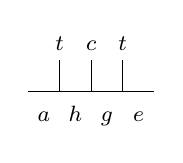
\begin{tikzpicture}[scale=0.4,font=\footnotesize,anchor=mid,baseline={([yshift=-.5ex]current bounding box.center)}]
        \draw (1, 0) to (1, -1);
        \draw (2, 0) to (2, -1);
        \draw (3, 0) to (3, -1);
        \node at (1, 0.5) {$t$};
        \node at (2, 0.5) {$c$};
        \node at (3, 0.5) {$t$};
        \draw (0, -1) to (4, -1);
        \node at (0.5, -1.75) {$a$};
        \node at (1.5, -1.75) {$h$};
        \node at (2.5, -1.75) {$g$};
        \node at (3.5, -1.75) {$e$};
      \end{tikzpicture}.
    \end{aligned}
  \end{equation}
\end{theorem*}

The Fibonacci anyons, defined by the fusion rules
\begin{equation}
  1 \times 1 = 1, \quad
  1 \times τ = τ \times 1 = τ, \quad
  τ \times τ = 1 + τ,
\end{equation}
were studied and we characterized the exchange operator $Uₚ$ explicitly in \cref{thm:fibonacci U_p}:
\begin{theorem*}
  Exchange of a pair of $τ$ anyons around $p$ enclosed $τ$ anyons introduces a non-abelian anyonic phase $U_p$, given by
  \begin{equation}
    \begin{aligned}
      U_0 &= ρ_2(σ_1) \\
      U_1 &= ρ_3(σ_1) ρ_3(σ_2) ρ_3(σ_1) \\
      U_p &= U_0^{\oplus\Fib(p-1)} \oplus U_1^{\oplus\Fib(p)}, \quad p \ge 2
    \end{aligned}
  \end{equation}
  expressed in the fused basis \cref{eq:F U_p basis}. The components are given by
  \begin{equation}
    \begin{aligned}
      U_0 &= R_{ττ}^1 \oplus R_{ττ}^τ \oplus R_{ττ}^τ \oplus B \\
      U_1 &= \left( R_{ττ}^τ \right)^3 \oplus \left( RBR \right) \oplus \left( BRB \right)
      \oplus \\
      & \oplus
      \begin{pmatrix}
        R_{\tau\tau}^\tau \left(B_{11}\right)^2+B_{12} B_{21} B_{22} & B_{12} B_{21} R_{\tau\tau}^\tau & B_{12} \left(B_{22}\right)^2+B_{11} B_{12} R_{\tau\tau}^\tau \\
        B_{12} B_{21} R_{\tau\tau}^\tau & B_{11} \left(R_{\tau\tau}^\tau\right)^2 & B_{12} B_{22} R_{\tau\tau}^\tau \\
        B_{21} \left(B_{22}\right)^2+B_{11} B_{21} R_{\tau\tau}^\tau & B_{21} B_{22} R_{\tau\tau}^\tau & \left(B_{22}\right)^3+B_{12} B_{21} R_{\tau\tau}^\tau
      \end{pmatrix}
    \end{aligned}
  \end{equation}
  where $R$ and $B$ are given in \cref{eq:fib F R,eq:fib F R B}, and below.
\end{theorem*}

We used this to draw conclusions regarding statistical repulsion for Fibonacci anyons. The above theorem allowed us to easily compute the spectrum of $Uₚ$ for Fibonacci anyons in \cref{res:Up fib} as
\begin{equation}
  \sigma(U_p) =
  \left\{
  \begin{array}{rl}
    e^{i4π/5}  &\text{\rm with multiplicity }\,\; \Fib(p+3), \\
    e^{iπ/5}   &\text{\rm with multiplicity }\,\; 2\Fib(p), \\
    e^{-iπ/5}  &\text{\rm with multiplicity }\,\; 3\Fib(p), \\
    e^{-i3π/5} &\text{\rm with multiplicity }\,\; 3\Fib(p-1)
  \end{array}
  \right\}
\end{equation}
for all $p$. From this the constant $λ_{0,p}²$ of the lower bound \cref{eq:summary lower bound} was computed
\begin{equation}
  λ_{0,p}² = \begin{cases}
    (3/5)², & p = 0, \\
    (1/5)², & p ≥ 1,
  \end{cases}
\end{equation}
showing that it may be energetically favorable for Fibonacci anyons to encircle other Fibonacci anyons. This can be theorized as implying some sort of clustering phenomenon. However, such phenomenon has not been confirmed in even in the case of abelian anyons.

If the Fibonacci anyons are considered to be static and have controllable position, they may in principle be used to perform quantum computation. We showed this by observing that the fusion space $V_{τ⁴}¹$ is two dimensional, just as required for a qubit.  Motivated by this, one defined Fibonacci qubits as
\begin{equation}
  \ket{0} \coloneqq \fs{τ,τ,τ,τ}{1,τ,1,τ,1}, \quad
  \ket{1} \coloneqq \fs{τ,τ,τ,τ}{1,τ,τ,τ,1}.
\end{equation}
We showed how quantum gates can be implemented by braiding the Fibonacci anyons. The representation of the braid group generators of the fusion space $V_{τ⁴}¹$ is given by
\begin{equation}
  ρ(σ_1) = R,\quad
  ρ(σ_2) = B,\quad
  ρ(σ_3) = R
\end{equation}
as shown in \cref{res:fibonacci qubit braiding}, where
\begin{equation}
  R =
  \begin{pmatrix}
    e^{-4πi/5} & 0 \\
    0 & e^{3πi/5}
  \end{pmatrix}, \quad
  B =
  \begin{pmatrix}
    φ^{-1}e^{-4πi/5} & φe^{3πi/5} \\
    φe^{3πi/5} & - φ^{-1}
  \end{pmatrix}.
\end{equation}
This describes how the state of Fibonacci qubits are changed when the $τ$-anyons are braided. Furthermore, Fibonacci anyons can be combined to give multi-qubit systems, thus being able to perform general quantum computation.

Possible continuation of this work is to improve the machinery for non-abelian statistics. Possibly gaining sharper bounds by considering the global nature of non-abelian states. For example, studying the Ising anyons in detail would also be a good next step, and compare to the case of Fibonacci anyons. Taking this further, a general explicit characterization of the spectrum of $Uₚ$ for general anyon models would be desirable.
